%%%%%%%%%%%%%%%%%%%%%%%%%%%%%%%%%%%%%%%%%%%%%%%%%%%%%%%%%%%%%%%%%%%%%%%%%%%
%
% Template for a LaTex article in English.
%
%%%%%%%%%%%%%%%%%%%%%%%%%%%%%%%%%%%%%%%%%%%%%%%%%%%%%%%%%%%%%%%%%%%%%%%%%%%

\documentclass[10pt,a4paper]{article}

% AMS packages:
\usepackage{amsmath, amsthm, amsfonts}
\usepackage{hyperref}
\usepackage[width=0.00cm, height=0.00cm, left=1.00cm, right=1.00cm, top=1.00cm, bottom=1.00cm]{geometry}
\usepackage{natbib}
\usepackage{graphicx}


% Theorems
%-----------------------------------------------------------------
\newtheorem{thm}{Theorem}[section]
\newtheorem{cor}[thm]{Corollary}
\newtheorem{lem}[thm]{Lemma}
\newtheorem{prop}[thm]{Proposition}
\theoremstyle{definition}
\newtheorem{defn}[thm]{Definition}
\theoremstyle{remark}
\newtheorem{rem}[thm]{Remark}

% Shortcuts.
% One can define new commands to shorten frequently used
% constructions. As an example, this defines the R and Z used
% for the real and integer numbers.
%-----------------------------------------------------------------
\def\RR{\mathbb{T}}
\def\ZZ{\mathbb{Z}}


% Similarly, one can define commands that take arguments. In this
% example we define a command for the absolute value.
% -----------------------------------------------------------------
\newcommand{\abs}[1]{\left\vert#1\right\vert}
\newcommand{\norm}[1]{\vert\vert#1\vert\vert}
\newcommand{\lamb}{$\lambda$}

% Operators
% New operators must defined as such to have them typeset
% correctly. As an example we define the Jacobian:
% -----------------------------------------------------------------
\DeclareMathOperator{\Jac}{Bc}

%-----------------------------------------------------------------
\title{Reinformcement Learning Theory Learning}
\author{Yue Wang}

\begin{document}
	\maketitle
	
	\abstract{	a simple note for RL theroy}
	
	\section{Introduction}
	\label{introduction}
	
	RL theory is very long history and these days
	
	\begin{itemize}
		\item Bullet point one
		\item Bullet point two
	\end{itemize}
	
	\begin{enumerate}
		\item Numbered list item one
		\item Numbered list item two
	\end{enumerate}
	
	\section{Notation and Formatting}
	\label{notation}
	some notations: 
	
	\begin{center}
		\begin{tabular}{ |c  c| } 
			\hline
			$ \mathcal{S} $ &    the state space \\ 
			$ \mathcal{A} $& the action space\\
			&\\
		
			$ s_t $ &    the state at time t, actual  \\ 
			$ s $ & the state\\
			&\\
			
		
			$ r_t $ & the reward at time t, actual\\
			$ r(s,a,s') $ & the reward from stat s take action to stat $s'$;\\
			&\\
			$ v_k(s) $ & the value of stat s at k iteration\\ 
			$ v_k $ & the value function at time k iteration\\
			
			&\\
			$p(s,a,s')$& the probability of transfer to $s'$ when given the current stat s and action a\\
				
			$p(\pi,s,a,s')$&the probability of transfer to $s'$ when given the current stat s and policy $\pi$\\	
			
			&\\
			
			$\pi$& the policy\\
			$\pi(s,a)$& the probability of take action a given the current stat s under policy $\pi$\\
			
			
			\hline
		\end{tabular}
	\end{center}
	
	
	
	
	
	
	\section{RL algorithms}
	\label{algorithms}
	
	\section{RL convergence theory}
	\label{convergence}
	
	\subsection{counterexample}	
	
	There are many  that shows the RL algorithms may not convergence even divergence under some conditions
	
	
	 In \citep[chap 11.3]{sutton2011reinforcement} the authors give  an intuitive conclusion about when these algorithms will divergence :
	 
	\begin{quotation}
		\em
		The danger of instability and divergence arises whenever we combine  three things:
		\begin{enumerate}
			\item training on a distribution of trainsition other than that naturally generated by the process whose expectation is being estimated(e.g. off-policy learning)
			\item scalable function approximation (e.g. linear semi-gradient)
			\item bootstrapping (eg, DP,TD learning)
		\end{enumerate}
	\end{quotation}
	
	There are many counter example, follows are some of that.
	
	\subsubsection{counterexample1}
	In \citep{Baird}  the author gives an example to show that the TD(0) algorithms with linear function approximation will diverge.

	\subsubsection{conberexample2}
	In \citep{bertsekas1995counterexample} the author gives an example to show that the \textbf{TD(\lamb) algorithm with linear function approximation }  convergence to a very poor approximation to the cost function.
	
	As showed in \ref{bertsekas}
		\begin{figure} 
			\centering
			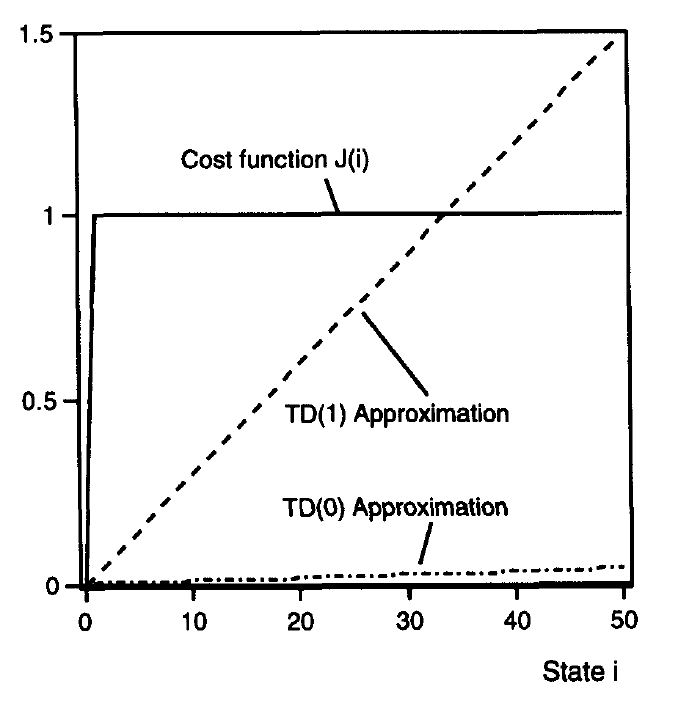
\includegraphics[width=1.77in,height=1.75in]{../graph/Bertsekas1.jpg}
			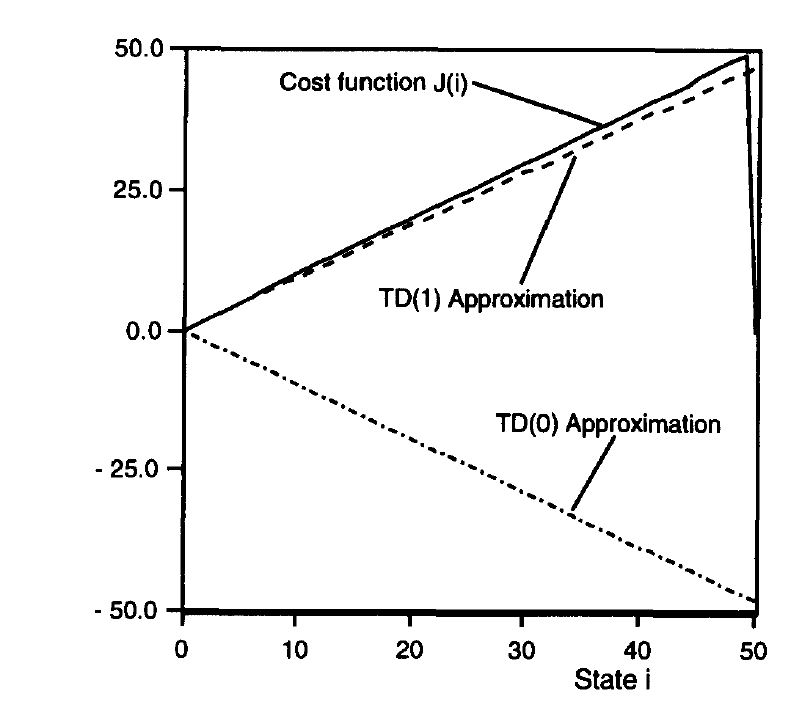
\includegraphics[width=1.87in,height=1.75in]{../graph/Bertsekas2.jpg}
			\caption{Bertsekas' counterexample}
			\label{bertsekas}
		\end{figure}
		
		
	\subsubsection{counterexample3}
	In \cite{Tsitsiklis1996} the author gives an example to show that the value iteration with linear function approximation use off policy may diverge
	

	\subsection{convergence for look up table}
	
		\subsubsection{policy iteration with look up table}


		\fbox{ 
			\parbox{\textwidth}{ 
				\begin{center}  
				\textbf{updata rule of policy iteration:}
				\end{center} 
 				\begin{description}
 					\item[evaluation:]  $ v_\pi = r(s,a,s')+\gamma\sum\limits_{a,s'}P(\pi,s,a,s')v_\pi(s') $
 					\item[improvement:] $ \pi_v(s)=\arg\max\limits_a(r(s,a,s')+\gamma\sum\limits_{s'}P(s,a,s')v_\pi(s') )$

 				\end{description}


			}  
		}  
		
		 \vspace{3ex}
		
		The proof of policy iteration :	
		
			
		First, prove the monotonicity of policy improvement
		
		
		Second, it is obvious that the number of policy is finite 
		
		\subsubsection{value iteration with look up table}
		
			\fbox{ 
				\parbox{\textwidth}{ 
					\begin{center}  
						\textbf{updata rule of value iteration:}
					\end{center} 
					\begin{enumerate}
						\item $v_{k+1}(s) = \mathcal{T}(v_k)(s)$
						\item $ \mathcal{T}(v_k)(s)=\max\limits_a[r(s,a,s')+\gamma\sum\limits_{s'}P(s,a,s')v_k(s')]$
						
					\end{enumerate}
					
					
				}  
			} 
		
		\vspace{3ex}
		
		The proof of  value iteration\cite{Tsitsiklis1996}:\\ $\norm{v_{k+1}-v^*}_\infty=\norm{\mathcal{T}(V_k)-\mathcal{T}(v^*)_\infty}\le\gamma\norm{v_k-v^*}_\infty\le\cdots\le\gamma^{k+1}\norm{v_0-v^*}_\infty\to 0$
		
		
		
		\subsubsection{Q-learning with look up table}
		
		
			\fbox{ 
				\parbox{\textwidth}{ 
					\begin{center}  
						\textbf{updata rule of Q-learning:}
					\end{center} 
					\begin{itemize}
						\item $  q_{k+1}=(1-\alpha)q_k(s_t,a_t)+\alpha\max\limits_b[r_t+\gamma q_k(s_{t+1},b)] $
						
						
					\end{itemize}
					
					
				}  
			} 
		
		\subsubsection{SARSA iteration with look up table}
		
		\fbox{ 
			\parbox{\textwidth}{ 
				\begin{center}  
					\textbf{updata rule of Q-learning:}
				\end{center} 
				\begin{itemize}
					\item $  q_{k+1}=(1-\alpha)q_k(s_t,a_t)+\alpha[r_t+\gamma q_k(s_{t+1},a_{t+1})] $
					
					
				\end{itemize}
				
				
			}  
		} 
		
	
	
	\subsection{convergence for linear function approximation}
	
		\subsubsection{linear function approximation with prediction problem}
		
		\subsubsection{linear function approximation with control problem}
	
	\subsection{convergence for nonlinear function approximation}	
		\subsubsection{nonlinear function approximation with prediction problem}
		
		\subsubsection{nonlinear function approximation with prediction problem}
	
	
	% Bibliography
	%-----------------------------------------------------------------
		\bibliographystyle{plainnat}
		%\bibliographystyle{ieeetr}
		\bibliography{../ref/sample,../ref/counterexample}
	
	
\end{document}